% Generated by jats2tex@0.11.1.0
\documentclass{article}
\usepackage[T1]{fontenc}
\usepackage[utf8]{inputenc} %% *
\usepackage[portuges,spanish,english,german,italian,russian]{babel} %% *
\usepackage{amstext}
\usepackage{authblk}
\usepackage{unicode-math}
\usepackage{multirow}
\usepackage{graphicx}
\usepackage{etoolbox}
\usepackage{xtab}
\usepackage{enumerate}
\usepackage{hyperref}
\usepackage{penalidades}
\usepackage[footnotesize,bf,hang]{caption}
\usepackage[nodayofweek,level]{datetime}
\usepackage[top=0.85in,left=2.75in,footskip=0.75in]{geometry}
\newlength\savedwidth
\newcommand\thickcline[1]{\noalign{\global
\savedwidth
\arrayrulewidth
\global\arrayrulewidth 2pt}
\cline{#1}
\noalign{\vskip\arrayrulewidth}
\noalign{\global\arrayrulewidth\savedwidth}}
\newcommand\thickhline{\noalign{\global
\savedwidth\arrayrulewidth
\global\arrayrulewidth 2pt}
\hline
\noalign{\global\arrayrulewidth\savedwidth}}
\usepackage{lastpage,fancyhdr}
\usepackage{epstopdf}
\pagestyle{myheadings}
\pagestyle{fancy}
\fancyhf{}
\setlength{\headheight}{27.023pt}
\lhead{
\includegraphics[width=10mm]{logo.png}}
\rhead{\ifdef{\journaltitle}{\journaltitle}{}
\ifdef{\volume}{vol.\,\volume}{}
\ifdef{\issue}{(\issue)}{}
\ifdef{\fpage}{\fpage--\lpage\,pp.}}
\rfoot{\thepage/\pageref{LastPage}}
\renewcommand{\footrule}{\hrule height 2pt \vspace{2mm}}
\fancyheadoffset[L]{2.25in}
\fancyfootoffset[L]{2.25in}
\lfoot{\sf \ifdef{\articledoi}{\articledoi}{}}
\setmainfont{Linux Libertine O}
\renewcommand*{\thefootnote}{\alph{footnote}}
\makeatletter
\newcommand{\fn}{\afterassignment\fn@aux\count0=}
\newcommand{\fn@aux}{\csname fn\the\count0\endcsname}
\makeatother

\newcommand{\journalid}{Rev Bras Epidemiol}
\newcommand{\publisherid}{rbepid}
\newcommand{\journaltitle}{Revista Brasileira de Epidemiologia}
\newcommand{\abbrevjournaltitle}{Rev. bras. epidemiol.}
\newcommand{\issnppub}{1415-790X}
\newcommand{\issnepub}{1980-5497}
\newcommand{\publishername}{Associação Brasileira de Pós -Graduação em Saúde
Coletiva}
\newcommand\articledoi{\textsc{doi} 10.1590/1980-5497201600002000}
\def\subject{\textsc{errata}}\newcommand{\subtitlestyle}[1]{-- \emph{#1}\medskip}
\newcommand{\transtitlestyle}[1]{\par\medskip\Large #1}
\newcommand{\transsubtitlestyle}[1]{-- \Large\emph{ #1}}

\newcommand{\titlegroup}{
\ifdef{\subtitle}{\subtitlestyle{\subtitle}}{}
\ifdef{\transtitle}{\transtitlestyle{\transtitle}}{}
\ifdef{\transsubtitle}{\transsubtitlestyle{\transsubtitle}}{}}

\title{\textsc{errata}\titlegroup{}}
\date{ 2016}
\def\volume{19}
\def\issue{02}
\def\fpage{469}
\def\lpage{470}
\def\permissions{Este é um artigo publicado em acesso aberto sob uma licença
Creative Commons}

\begin{document}
\selectlanguage{portuges}
\section*{Metadados não aplicados}
\begin{itemize}
\item[\textbf{língua do artigo}]{Português}
\ifdef{\journalid}{\item[\textbf{journalid}] \journalid}{}
\ifdef{\journaltitle}{\item[\textbf{journaltitle}] \journaltitle}{}

\ifdef{\journalsubtitle}{\item[\textbf{journalsubtitle}] \journaltitle}{}
\ifdef{\transjournaltitle}{\item[\textbf{journaltitle}] \journaltitle}{}
\ifdef{\transjournalsubtitle}{\item[\textbf{journalsubtitle}] \journaltitle}{}

\ifdef{\abbrevjournaltitle}{\item[\textbf{abbrevjournaltitle}]
\abbrevjournaltitle}{}
\ifdef{\issnppub}{\item[\textbf{issnppub}] \issnppub}{}
\ifdef{\issnepub}{\item[\textbf{issnepub}] \issnepub}{}
\ifdef{\publishername}{\item[\textbf{publishername}] \publishername}{}
\ifdef{\publisherid}{\item[\textbf{publisherid}] \publisherid}{}
\ifdef{\subject}{\item[\textbf{subject}] \subject}{}
\ifdef{\transtitle}{\item[\textbf{transtitle}] \transtitle}{}
\ifdef{\authornotes}{\item[\textbf{authornotes}] \authornotes}{}
\ifdef{\articleid}{\item[\textbf{articleid}] \articleid}{}
\ifdef{\articledoi}{\item[\textbf{articledoi}] \articledoi}{}
\ifdef{\volume}{\item[\textbf{volume}] \volume}{}
\ifdef{\issue}{\item[\textbf{issue}] \issue}{}
\ifdef{\fpage}{\item[\textbf{fpage}] \fpage}{}
\ifdef{\lpage}{\item[\textbf{lpage}] \lpage}{}
\ifdef{\permissions}{\item[\textbf{permissions}] \permissions}{}
\end{itemize}
\maketitle

No artigo "Frequência do uso de narguilé em adultos e sua distribuição conforme
características sociodemográficas, moradia urbana ou rural e unidades
federativas: Pesquisa Nacional de Saúde (\textsc{pns}), 2013", com número de \textsc{doi}:
10.1590/1980-5497201500060006, publicado no periódico Rev. bras. epidemiol.,
18(supl.2):57-67, nas páginas 62 e 63:

Onde se lia:

\begin{figure}
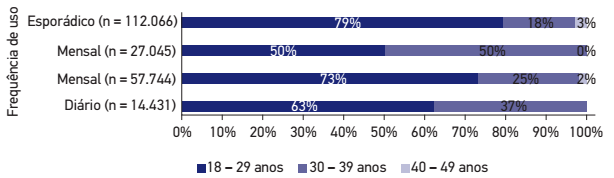
\includegraphics[width=\textwidth]{1980-5497-rbepid-19-02-00469-gf1.png}
\caption{}\label{fig:f1}
\end{figure}

Leia-se:

\begin{figure}
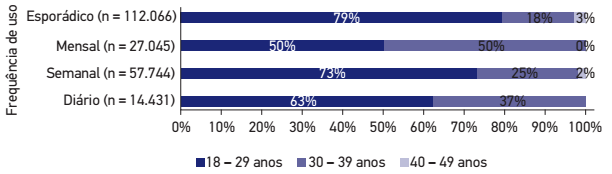
\includegraphics[width=\textwidth]{1980-5497-rbepid-19-02-00469-gf2.png}
\caption{}\label{fig:f2}
\end{figure}

Onde se lia:

\begin{figure}
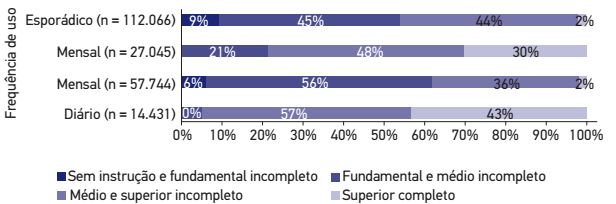
\includegraphics[width=\textwidth]{1980-5497-rbepid-19-02-00469-gf3.png}
\caption{}\label{fig:f3}
\end{figure}

Leia-se:

\begin{figure}
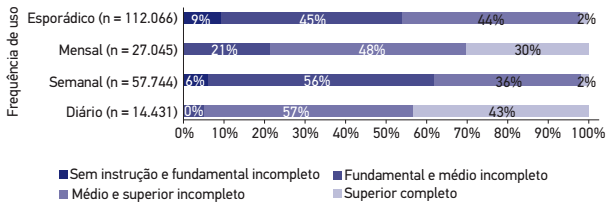
\includegraphics[width=\textwidth]{1980-5497-rbepid-19-02-00469-gf4.png}
\caption{}\label{fig:f4}
\end{figure}

\end{document}
